\documentclass{article}
\usepackage{amsmath}
\usepackage{fancyvrb,relsize}
\usepackage{graphicx}
\usepackage{listings}
\usepackage[bookmarks=true,bookmarksnumbered=true]{hyperref}

\setlength\topmargin{0in}
\setlength\headheight{0in}
\setlength\headsep{0in}
\setlength\textheight{7.7in}
\setlength\textwidth{6.5in}
\setlength\oddsidemargin{0in}
\setlength\evensidemargin{0in}
\setlength\parindent{0.25in}
\setlength\parskip{0.25in} 


\begin{document}

\lstset{showspaces=false, showstringspaces=false,
  showtabs=false, frame=single, basicstyle=\small}
\title{Creating mixed FLASH/Chombo applications}
\author{Chris Daley}
\maketitle

\tableofcontents
%\listoftables
%\listoffigures
\clearpage


\section{Accessing the code}

The Chombo-dev svn branch is at the following location:

\begin{lstlisting}[language=TeX]
svn+ssh://USERNAME@flash.uchicago.edu/home/svn/repos/FLASH3/branches/Chombo-dev
\end{lstlisting}

There is also a svn vendor branch containing Chombo-3.0-Oct2009 at the
following location:

\begin{lstlisting}[language=TeX]
svn+ssh://USERNAME@flash.uchicago.edu/home/svn/repos/FLASH3/vendor/chomboForFlash
\end{lstlisting}

It is convenient to use this vendor branch because it contains Chombo
Makefiles for various Flash Center machines and a small patch to build
applications on Intrepid BG/P.


\section{Creating FLASH-Chombo applications}

The standard FLASH build system is used to create a mixed FLASH-Chombo
application.  The FLASH Makefile will link FLASH against the
appropriate dimensionality Chombo libraries and so Chombo must be
pre-built in 1D, 2D and 3D before building a mixed FLASH-Chombo
application.

A FLASH Config file registers Chombo as an external library to the
setup script and so the generated FLASH Makefile depends on the macros
CFLAGS\_\-CHOMBO and LIB\_\-CHOMBO.  The macro CFLAGS\_\-CHOMBO is
used when compiling the FLASH C++ code that interacts with Chombo
library and LIB\_\-CHOMBO is used to link against the Chombo
libraries.  Both macros must be defined by the user in
Makefile.h.chombo.  Figure \ref{Fig:MakefileVariables} shows the macro
values used on code.uchicago.edu.

\begin{figure}
\begin{lstlisting}[language=TeX]
CHOMBO_PATH = /home/cdaley/flash/chomboForFlash/current

_DIM = $(shell grep ``define NDIM'' Flash.h | cut -d `` `` -f 3)
_CPP = $(shell make vars DIM=${_DIM} -C ${CHOMBO_PATH}/lib | \
         awk -F 'CPPFLAGS=' '/^CPPFLAGS/{print $$2}')
_LIB = $(shell make vars DIM=${_DIM} -C ${CHOMBO_PATH}/lib | \
         awk -F 'config=' '/^config/{print $$2}')

CFLAGS_CHOMBO = -I${CHOMBO_PATH}/lib/include ${_CPP} -DCH_LANG_CC
LIB_CHOMBO = -L$(CHOMBO_PATH)/lib \
-lamrtimedependent${_LIB} \
-lamrtools${_LIB} \
-lboxtools${_LIB} \
-lbasetools${_LIB} \
-lstdc++
\end{lstlisting}
\caption{FLASH Makefile.h.chombo variables}
\label{Fig:MakefileVariables}
\end{figure}

The setup shortcuts +chombo\_ug and +chombo\_amr are available to build
UG and AMR FLASH applications respectively.  They correspond to:

\begin{lstlisting}[language=TeX]
chombo_ug:-unit=Grid/GridMain/Chombo/UG:-index-reorder:Grid=Chombo:-maxblocks=1:
-nofbs:-makefile=chombo:chomboCompatibleHydro=True

chombo_amr:-unit=Grid/GridMain/Chombo/AMR:-index-reorder:Grid=Chombo:
-nofbs:-makefile=chombo:chomboCompatibleHydro=True
\end{lstlisting}

\section{Available software stacks}

\begin{itemize}
\item GNU
  \begin{itemize}
  \item lenovolaptop
    \begin{itemize}
    \item sites/lenovolaptop/Makefile.h
    \item lib/chombo/lib/mk/local/Make.defs.lenovolaptop
    \end{itemize}
  \item archimedes
    \begin{itemize}
    \item sites/archimedes.uchicago.edu/Makefile.h
    \item lib/chombo/lib/mk/local/Make.defs.archimedes
    \end{itemize}
  \end{itemize}
\item Intel
  \begin{itemize}
  \item code
    \begin{itemize}
    \item sites/code.uchicago.edu/Makefile.h
    \item lib/chombo/lib/mk/local/Make.defs.code
    \end{itemize}
  \item mongchi
    \begin{itemize}
    \item sites/mongchi.uchicago.edu/Makefile.h
    \item lib/chombo/lib/mk/local/Make.defs.mongchi
    \end{itemize}
  \end{itemize}
\item XL
  \begin{itemize}
  \item intrepid
    \begin{itemize}
    \item sites/intrepid.alcf.anl.gov/Makefile.h
    \item lib/chombo/lib/mk/local/Make.defs.intrepid
    \end{itemize}
  \end{itemize}
\end{itemize}


NOTE: gfortran $>=4.4.2$ is required because there is a pointer
interoperability bug in earlier versions of gfortran.  See
\href{http://gcc.gnu.org/bugzilla/show_bug.cgi?id=40962}{\bf{GCC
    bugzilla 40962}}.

\section{Runtime parameters}

\subsection{Chombo UG}

\begin{itemize}
\item {\bf iGridSize, jGridSize, kGridSize:} The total number of grid
  points along each dimension of the global domain.
  
\item {\bf iProcs, jProcs, kProcs:} The total number of processors
  along each dimension of the global domain.
\end{itemize}


\subsection{Chombo AMR}

\begin{itemize}
\item {\bf iGridSize, jGridSize, kGridSize:} The total number of grid
  points along each dimension of the coarsest level.
  
\item {\bf lrefine\_max:} The unit-based maximum refinement level.  A
  value of 3 means that blocks can refine a maximum of 2 times.

\item {\bf flux\_correct:} Logical flag to turn on/off flux correction.
  Currently always off because flux correction is not yet implemented.

\item {\bf maxBlockSize:} The maximum FLASH block size.  In Chombo
  terminology this is the maximum grid size.

\item {\bf BRMeshRefineFillRatio:} See a\_fillRatio argument of 
  BRMeshRefine define method in Chombo user-guide.

\item {\bf BRMeshRefineBufferSize:} See a\_bufferSize argument of
  BRMeshRefine define method in Chombo user-guide.

\item {\bf BRMeshRefineBlockFactor:} See a\_blockFactor argument of
  BRMeshRefine define method in Chombo user-guide.  Note that setting 
  this parameter equal to {\bf maxBlockSize} leads to a mesh where 
  all blocks have the same number of cells.

\item {\bf tagRadius:} The radius of cells around a tagged cell that
  should also be tagged, i.e. marked for refinement

\end{itemize}


\section{Unit\_test}

There are unit tests in sub-directories 1 and 2 at the following
location in the Chombo-dev source tree:

\begin{lstlisting}[language=TeX]
source/Grid/GridMain/Chombo/wrapper/unit_tests
\end{lstlisting}


\subsection{1}
This test is independent of FLASH and Chombo.  It simply tests
interoperability of pointers in a serial, mixed Fortran/C++ code.
Note that this test will fail with versions of gfortran $< 4.4.2$
because the compiler introduces a pointer indexing bug (see GCC
bugzilla 40962).  Build with make [gnu, intel, ibm, sun].


\subsection{2}
This test depends on Chombo only.  It tests usage of Chombo library in
a parallel, mixed Fortran/C++ code.  The main() function is written in
Fortran and calls C++ functions that use Chombo to generate a
distributed uniform grid.  The application must be run with 4 MPI
processes.  Build with ./compile.sh [gnu, intel, ibm].


\section{Test problems}

\subsection{Sedov}

The standard FLASH Sedov explosion problem can be run with Chombo Grid
implementation.  The generated checkpoint files are in HDF5 format and
can be visualized using visit.  The following aliases may be useful.\\

\begin{lstlisting}[language=bash]
alias visit_flash='visit -assume_format FLASH'
alias visit_chombo='visit -assume_format Chombo'
\end{lstlisting}


\subsubsection{Uniform grid}
Creates a uniform grid with 1 box per MPI process.  The box
size is determined from igridsize,jgridsize,kgridsize and 
iprocs,jprocs,kprocs runtime parameters.\\

\begin{lstlisting}[language=TeX]
./setup Sedov -auto +chombo_ug -parfile=test_chombo_ug_2d.par
\end{lstlisting}


A grid size of $512^{2}$ is created for FLASH UG and Chombo UG and the
resulting application is run on 1024 cores of Intrepid.  The final
checkpoint file occurs at t=0.05 seconds and is visualized with visit.
Figures \ref{Fig:High_res_flash} and \ref{Fig:High_res_chombo} show
the generated pseudocolor plot of density mesh variable for FLASH UG
and Chombo UG.

\clearpage

\begin{figure}[!t]
\begin{center}
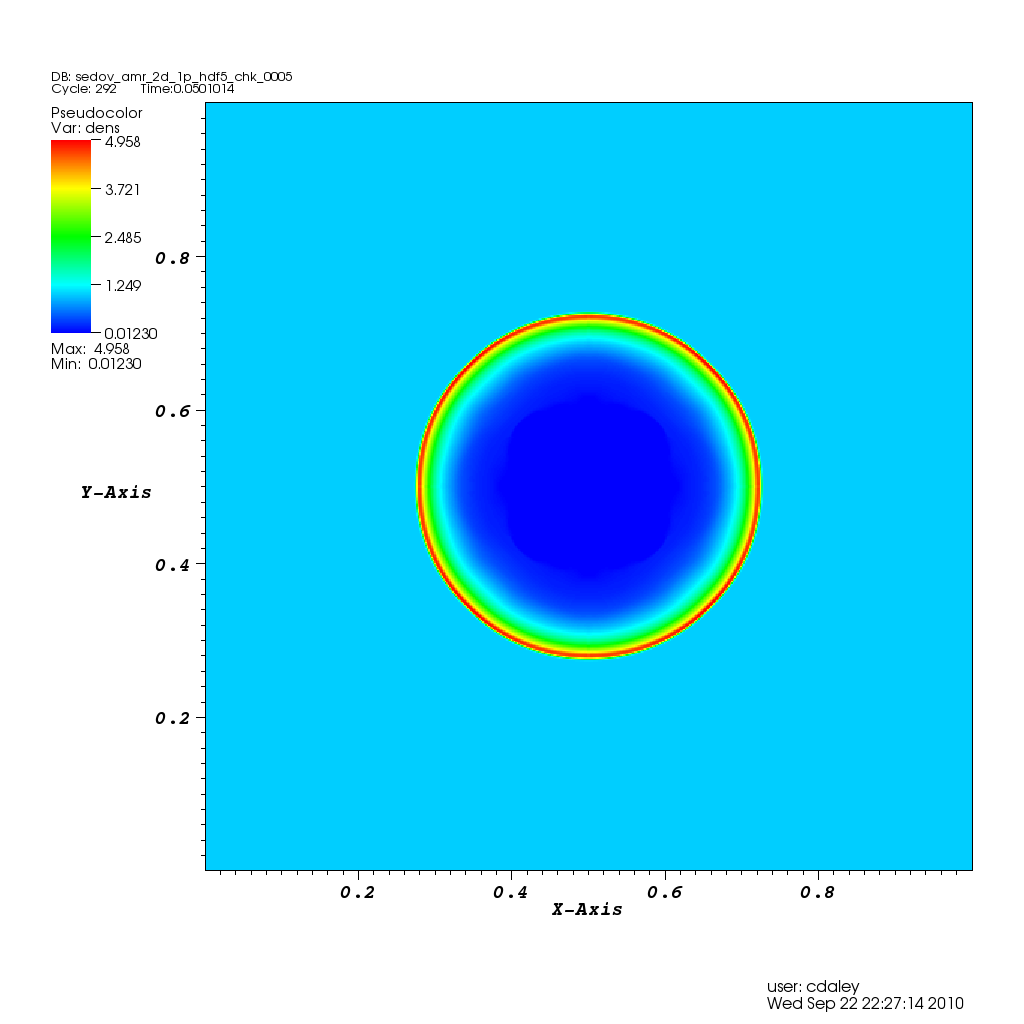
\includegraphics[scale=0.22]{figures/visit_flash}
\caption{High resolution Sedov application with NOFBS uniform grid}
\label{Fig:High_res_flash}
\end{center}
\end{figure}

\begin{figure}[!b]
\begin{center}
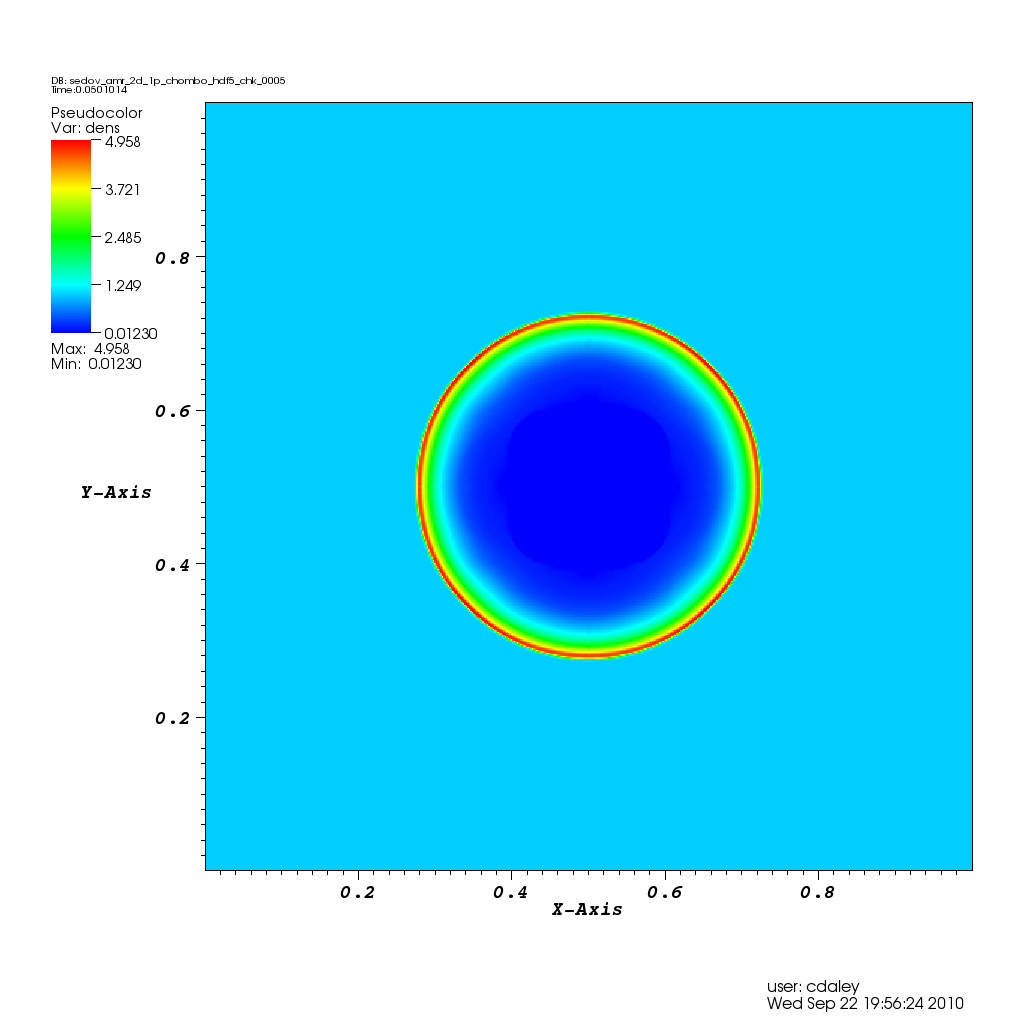
\includegraphics[scale=0.22]{figures/visit_chombo}
\caption{High resolution Sedov application with Chombo grid}
\label{Fig:High_res_chombo}
\end{center}
\end{figure}

\clearpage


\subsubsection{Adaptive grid}

The Sedov problem can also be run with a Chombo adaptive grid using
the following setup line:

\begin{lstlisting}[language=TeX]
./setup Sedov -auto +chombo_amr -parfile=test_chombo_amr_2d.par
\end{lstlisting}

The density mesh variable and Chombo patches are shown in Figure
\ref{Fig:SedovAMR} at 0.01 second intervals.  It can be seen that the
Chombo patches are clustered near the explosion front.  This
demonstrates that FLASH is able to communicate to Chombo the cells
that need to be tagged for refinement, however, there are some
anomolies with the clustering because the test problem is symmetrical.
This non-symmetry is most likely an issue with my custom
gr\_markRefineDerefine which is a hacked cell-based version of the
default block-based Paramesh gr\_markRefineDerefine.


\clearpage
\begin{figure}[h]
\begin{center}$
\begin{array}{cc}
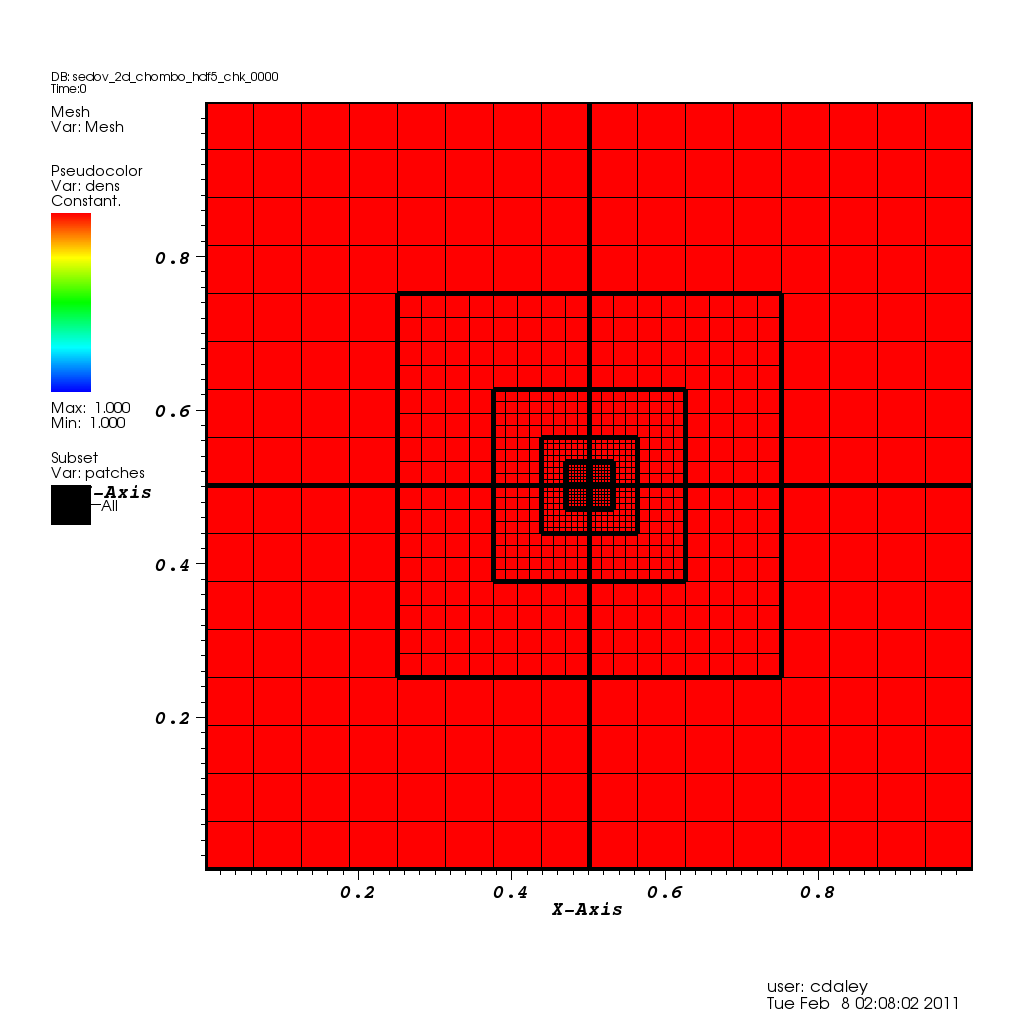
\includegraphics[width=2.2in]{figures/sedov_2d_chombo_hdf5_chk_0000.png} &
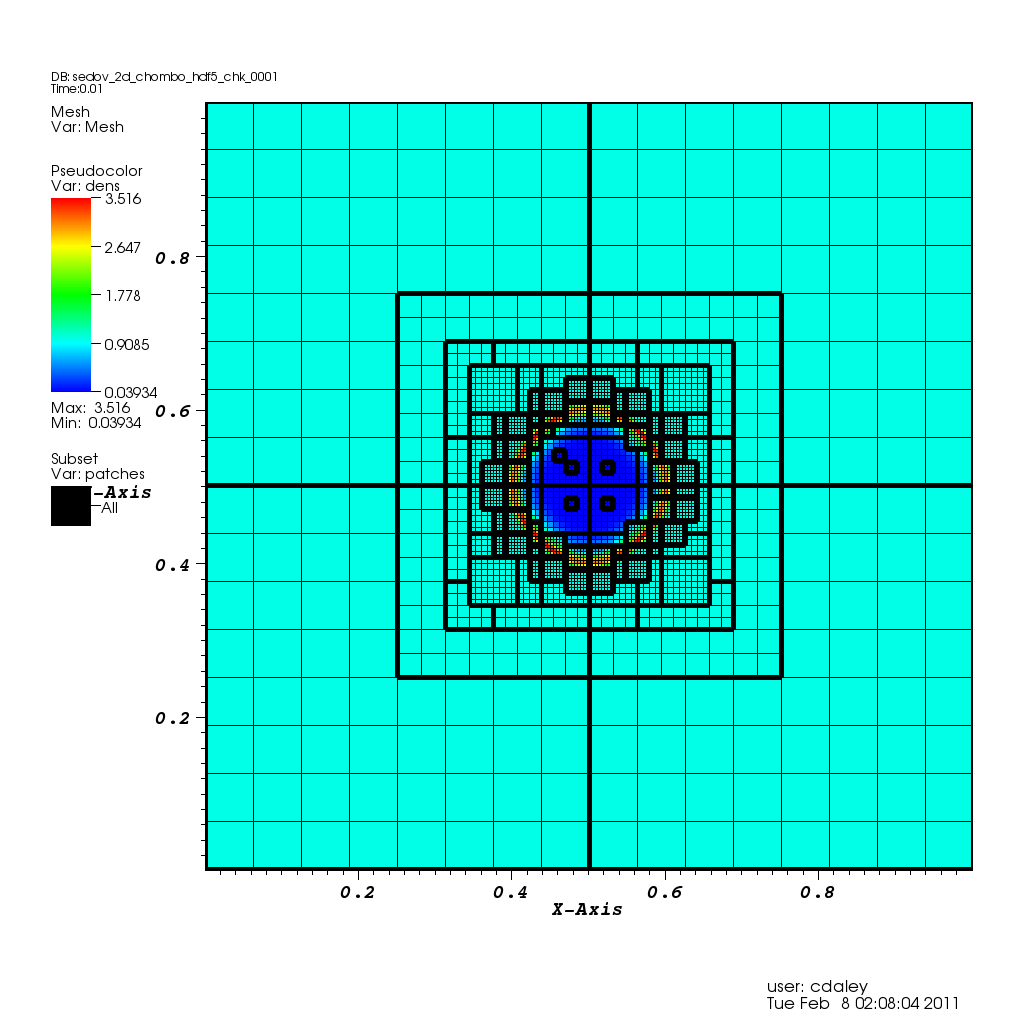
\includegraphics[width=2.2in]{figures/sedov_2d_chombo_hdf5_chk_0001.png} \\
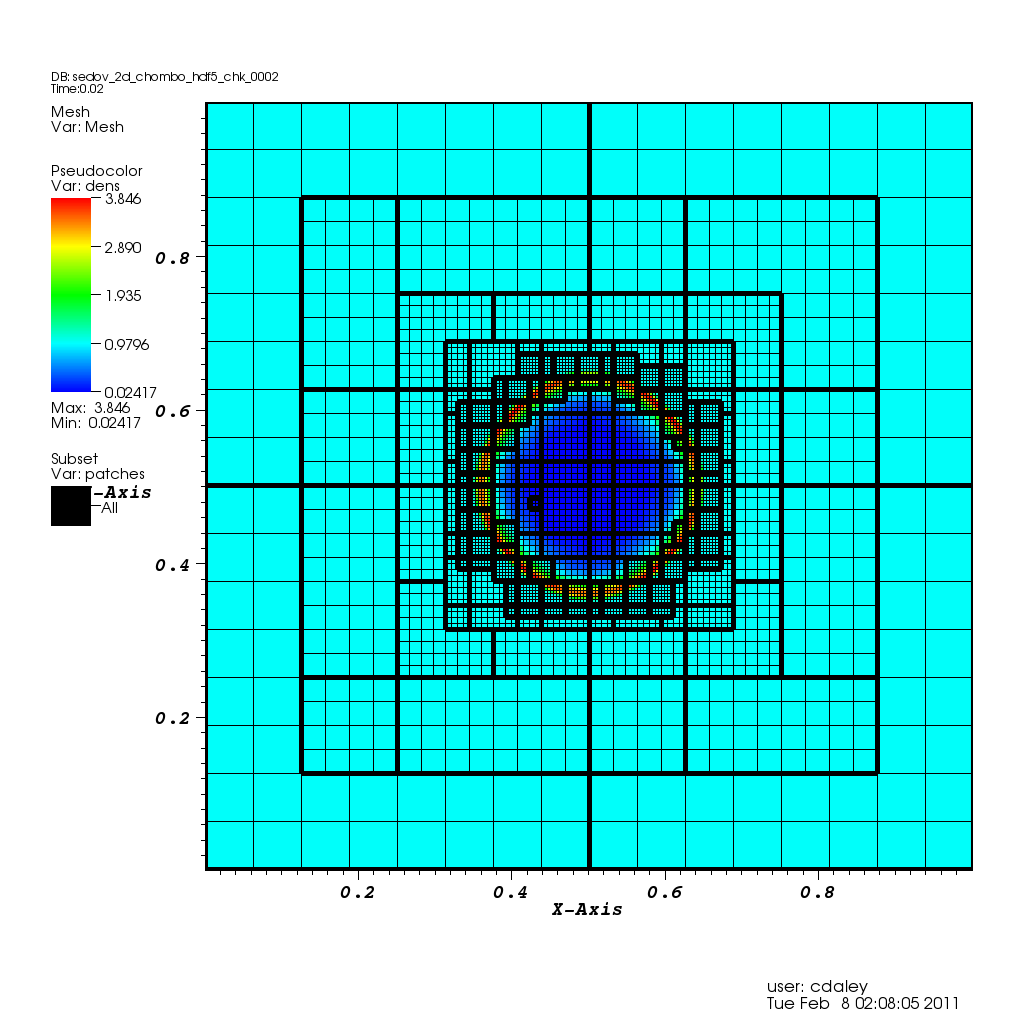
\includegraphics[width=2.2in]{figures/sedov_2d_chombo_hdf5_chk_0002.png} &
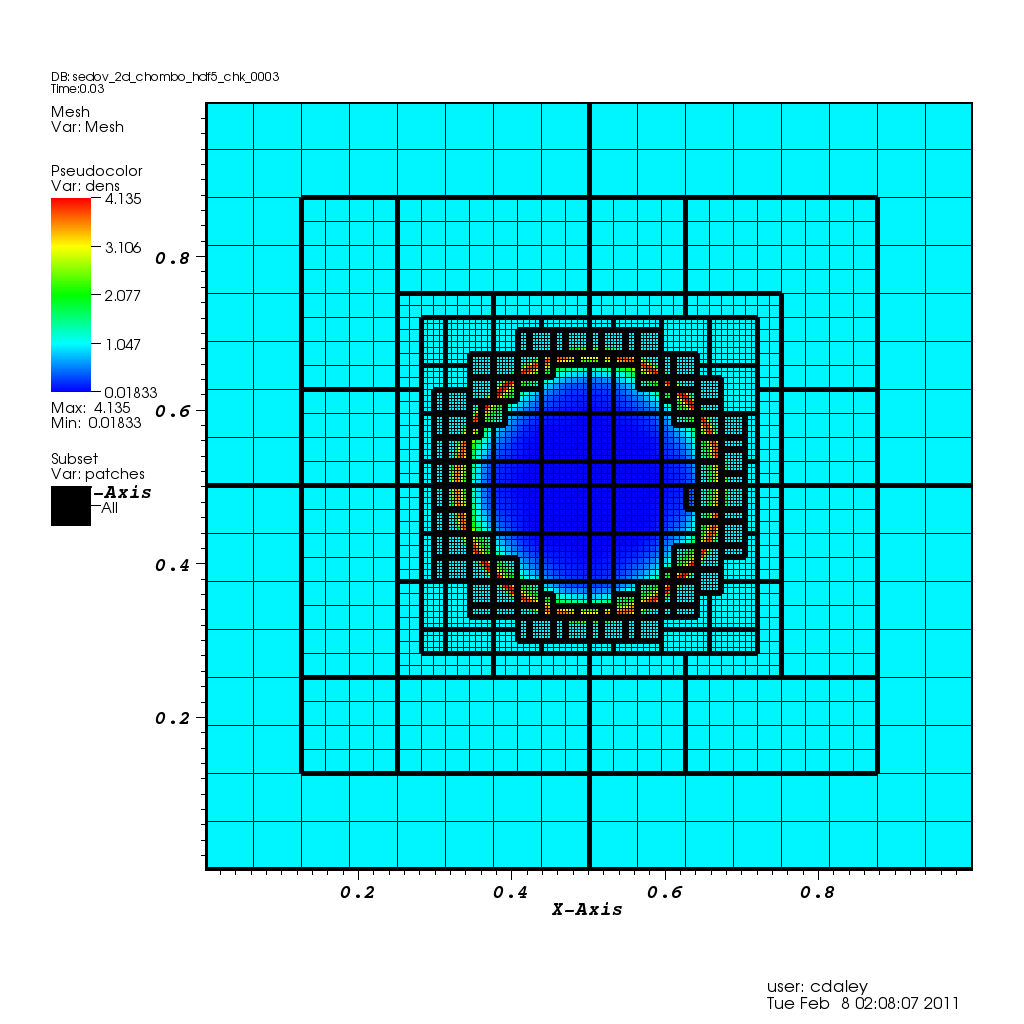
\includegraphics[width=2.2in]{figures/sedov_2d_chombo_hdf5_chk_0003.png} \\
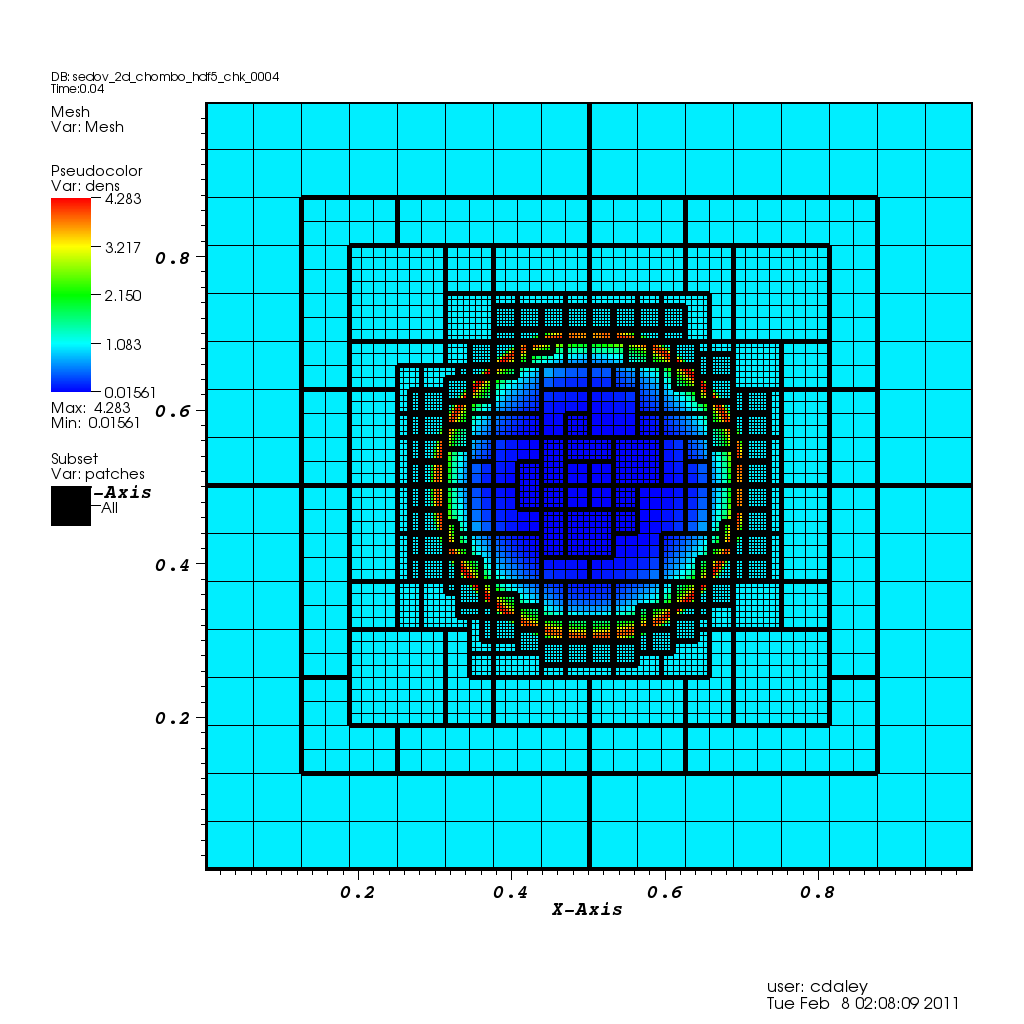
\includegraphics[width=2.2in]{figures/sedov_2d_chombo_hdf5_chk_0004.png} &
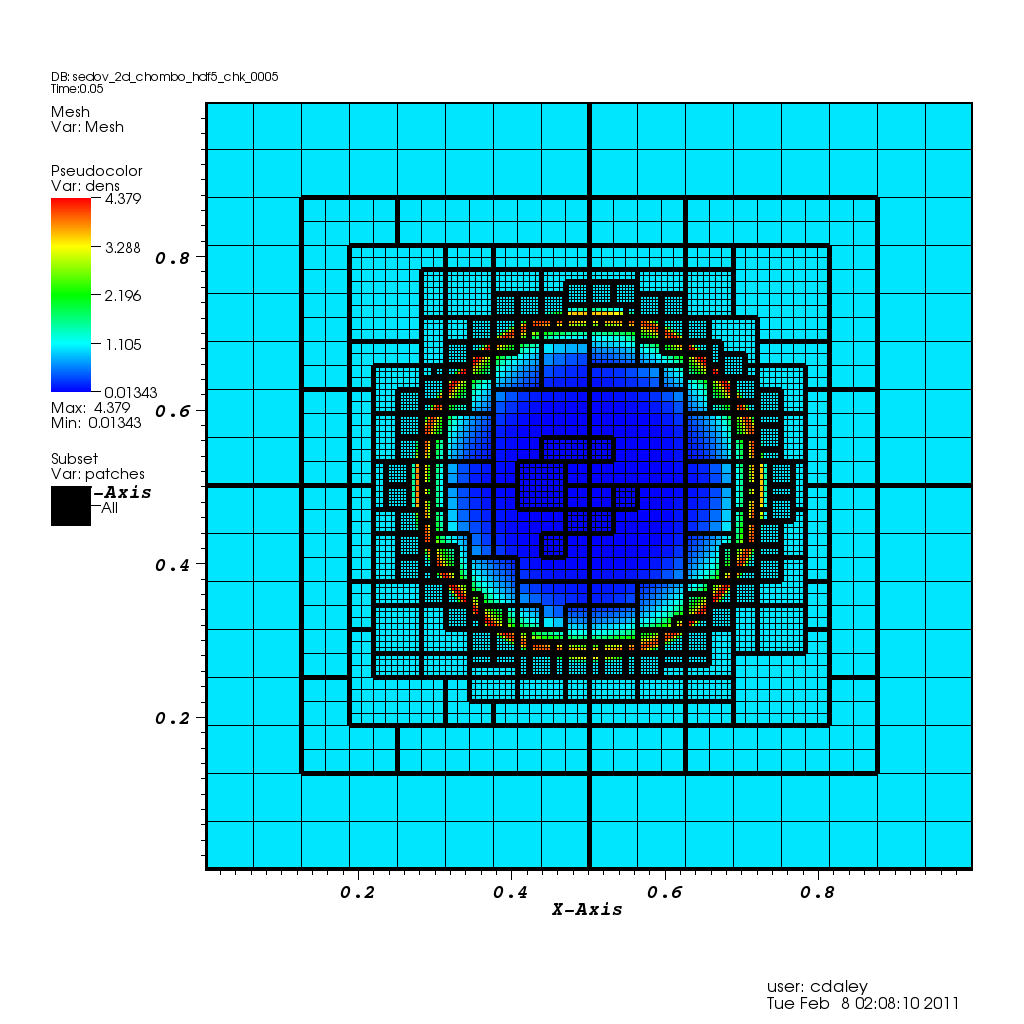
\includegraphics[width=2.2in]{figures/sedov_2d_chombo_hdf5_chk_0005.png}
\end{array}$
\end{center}
\caption{Density at 0.01 second intervals in a Sedov simulation using
  AMR capabilities of Chombo}
\label{Fig:SedovAMR}
\end{figure}
\clearpage

\subsection{Sod}
The FLASH Sod problem can be setup with split or unsplit Hydro 
using:

\begin{lstlisting}[language=TeX]
./setup Sod -auto +chombo_amr -parfile=test_chombo_amr_2d.par
./setup Sod -auto +chombo_amr +uhd -parfile=test_chombo_amr_2d.par
\end{lstlisting}

This problem tests the code's ability to capture shocks.  Originally
we had problems with non-convergence in Riemann solver.  We believe
the non-convergence was because of fine-coarse interpolation in a
region of the domain where there were steep gradients.

We overcame the non-convergence by tagging cells for refinement more
liberally; whenever we tagged a cell we also tagged nearest neighbor
cells up to a set distance.  This allows us to refine a region of the
domain (rather than a single cell) in preparation for an approaching
shock, and seems to avoid the fine-coarse interpolation issue.  The
default tag distance is 2 and is controlled by the parameter,
tagRadius.  The Sedov images above were obtained before we changed the
tagging code and so had a tag distance of 0.

The density mesh variable is shown at 0.04 second intervals in Figure
\ref{Fig:SodAMR}.

\clearpage
\begin{figure}[h]
\begin{center}$
\begin{array}{cc}
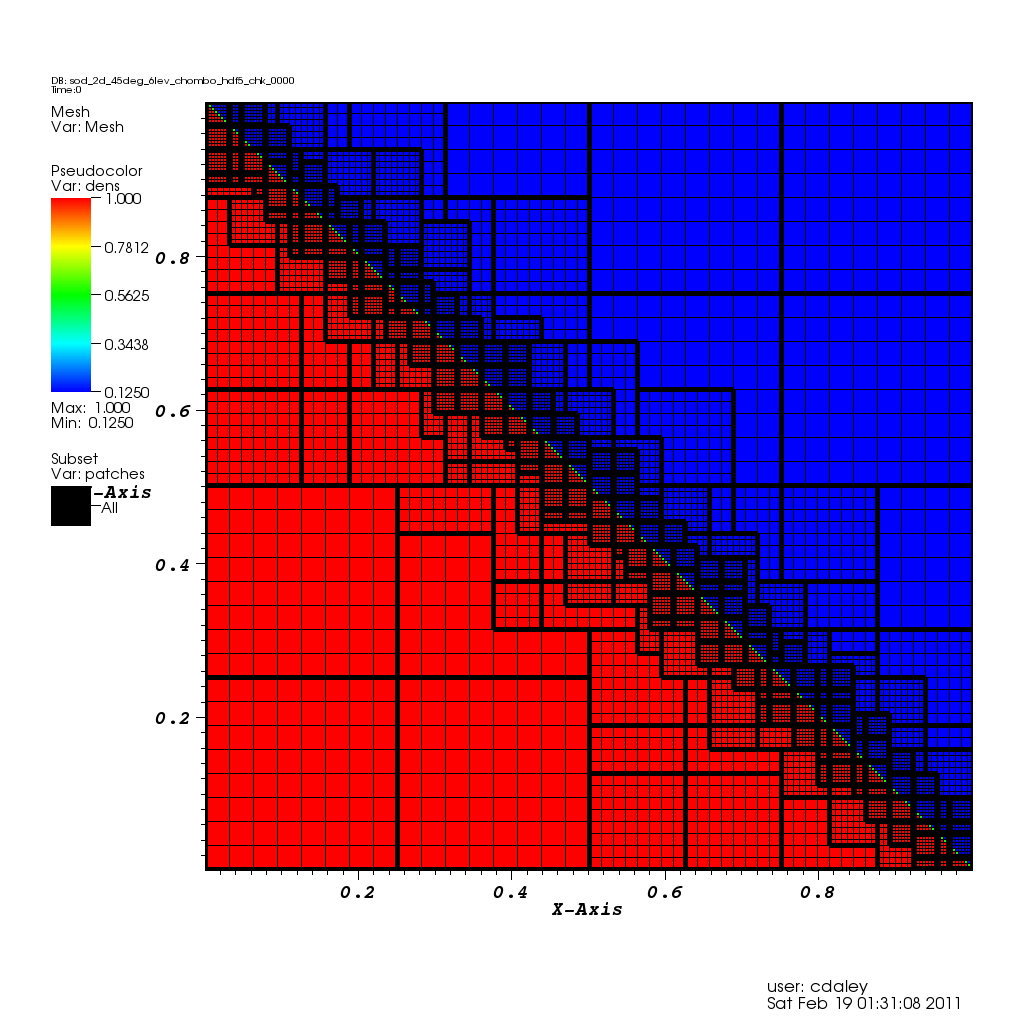
\includegraphics[width=2.2in]{figures/sod/sod_2d_45deg_6lev_chombo_hdf5_chk_0000.png} &
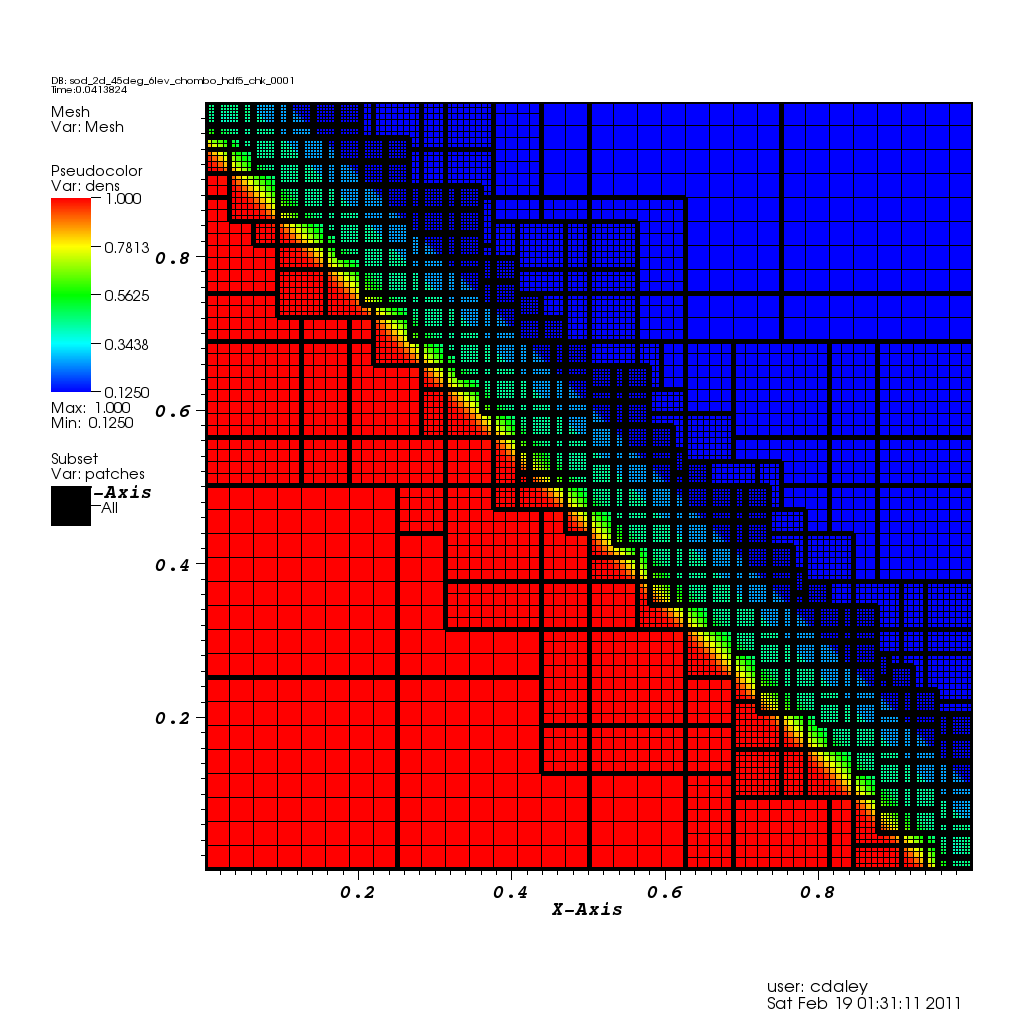
\includegraphics[width=2.2in]{figures/sod/sod_2d_45deg_6lev_chombo_hdf5_chk_0001.png} \\
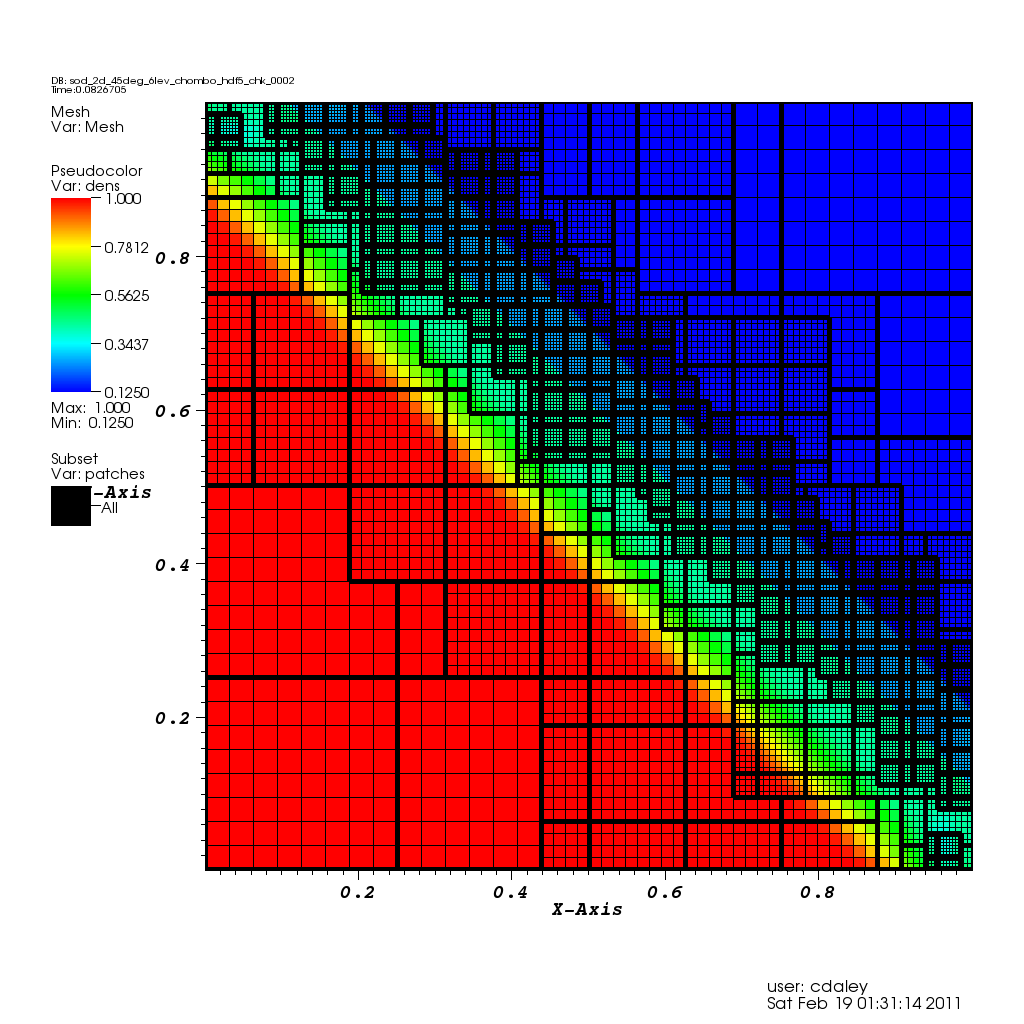
\includegraphics[width=2.2in]{figures/sod/sod_2d_45deg_6lev_chombo_hdf5_chk_0002.png} &
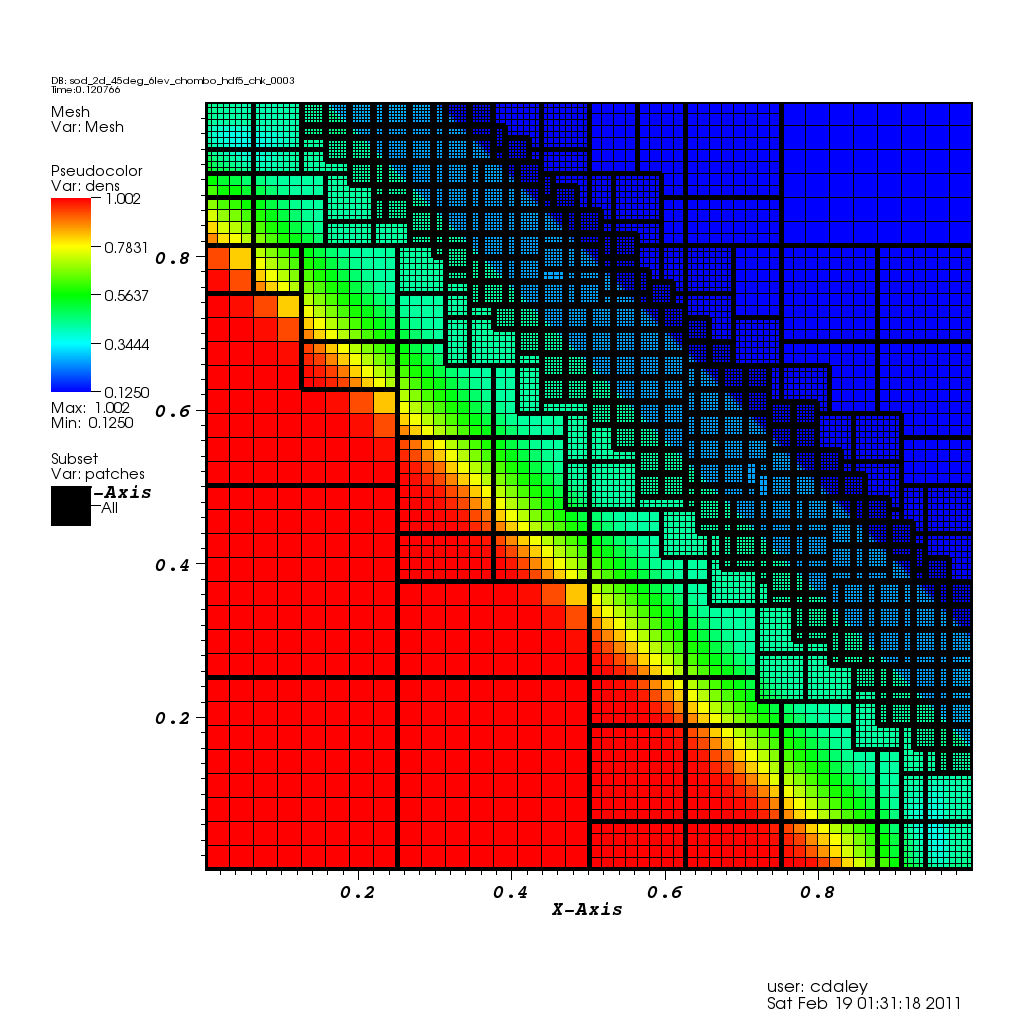
\includegraphics[width=2.2in]{figures/sod/sod_2d_45deg_6lev_chombo_hdf5_chk_0003.png} \\
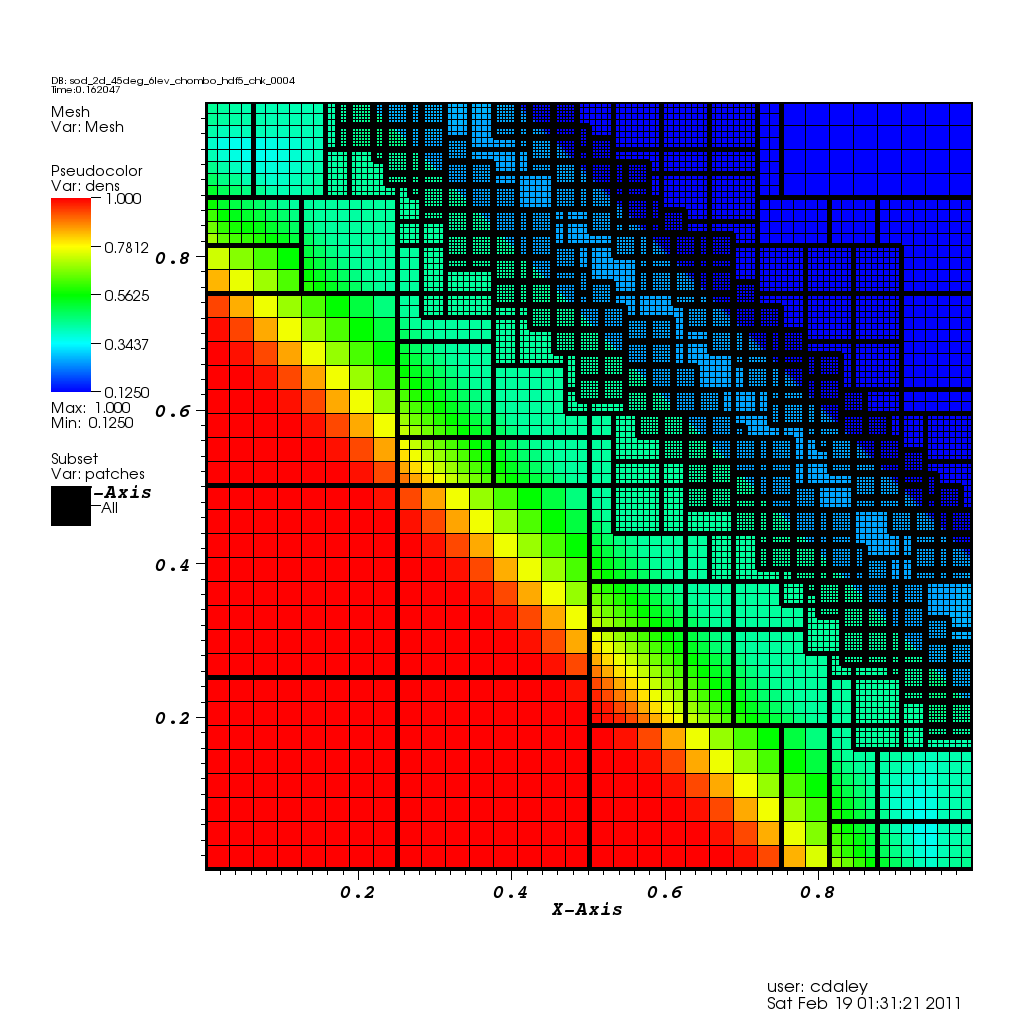
\includegraphics[width=2.2in]{figures/sod/sod_2d_45deg_6lev_chombo_hdf5_chk_0004.png} &
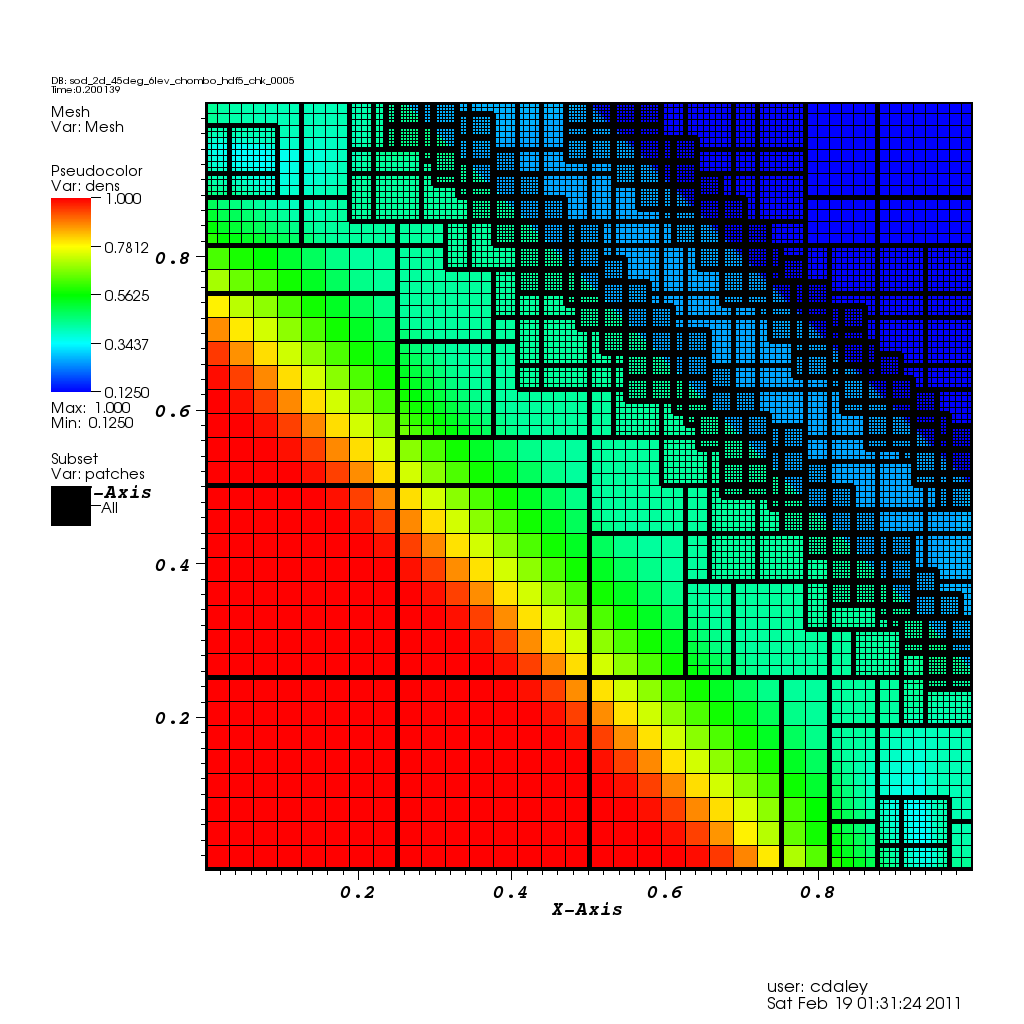
\includegraphics[width=2.2in]{figures/sod/sod_2d_45deg_6lev_chombo_hdf5_chk_0005.png}
\end{array}$
\end{center}
\caption{Density at 0.04 second intervals in a Sod simulation using
  AMR capabilities of Chombo}
\label{Fig:SodAMR}
\end{figure}
\clearpage


\subsection{Others}
The following unit tests work as expected:

\begin{lstlisting}[language=TeX]
setupName: unitTest/Eos/Multigamma
setupOptions: -auto -3d +chombo_amr +noio -debug
numProcs: 1
parfiles: <pathToSimulations>/unitTest/Eos/Multigamma/chombo_3d.par

setupName: unitTest/Eos/Multigamma
setupOptions: -auto -3d +chombo_ug +noio -debug
numProcs: 1
parfiles: <pathToSimulations>/unitTest/Eos/Multigamma/chombo_3d.par

setupName: unitTest/PFFT_PoissonFD
setupOptions: -auto -3d +chombo_ug +noio -debug
numProcs: 4
pathToParfiles: <pathToSimulations>/unitTest/PFFT_PoissonFD
parfiles: <pathToParfiles>/test_UG_4p_3d_16cube.par
          <pathToParfiles>/test_UG_4p_3d_32cube.par
          <pathToParfiles>/test_UG_4p_3d_64cube.par 
          <pathToParfiles>/test_UG_4p_3d_128cube.par
\end{lstlisting}

The following test problems run, but have been looked at less:

\begin{lstlisting}[language=TeX]
setupName: Blast2
setupOptions: -auto -1d +chombo_amr
numProcs: 4
parfiles: <pathToSimulations>/Blast2/test_chombo_amr_1d.par

setupName: IsentropicVortex
setupOptions: -auto -2d +chombo_amr
numProcs: 2
parfiles: <pathToSimulations>/IsentropicVortex/test_chombo_amr_2d.par

setupName: StirTurb
setupOptions: -auto -3d +chombo_amr
numProcs: 4
parfiles: <pathToSimulations>/StirTurb/test_chombo_amr_3d.par
\end{lstlisting}

\section{Design overview}

The FLASH Grid API subroutines call ``C'' linkage functions in
chombo\_f\_c\_api which in turn call methods on an object that
interacts with Chombo library.  There are two different objects for
interacting with Chombo library, either a chombo\_uniform\_grid (for
UG) or a chombo\_adaptive\_grid (for AMR).

The chombo\_uniform\_grid object is much simpler and only contains a
DisjointBoxLayout Chombo object and a LevelData$<$FArrayBox$>$ Chombo
object.  It provides identical functionality to a single box per MPI
process FLASH uniform grid.

The chombo\_adaptive\_grid object is much more complicated and
contains partial usage of Chombo's AMR framework.  As described in the
Chombo user-guide, the Chombo AMR framework consists an AMR object
calling methods on a user's object (which is instantiated from a class
that inherits from AMRLevel class).  In this framework the user's
AMRLevel class is expected to contain the data representation for one
level and also implement the algorithms for advancing one level in
time.

The derived AMRLevel class in FLASH does not contain any code for
advancing one level in time.  This does fit with the intended usage of
AMR framework in a Chombo application, but doing things this way
allows FLASH's Hydro unit to perform time advancement.  It is an abuse
of Chombo's AMR framework that allows re-use of nearly 1000 lines of
code from the example AMRLevel class named AMRLevelPolytropicGas.

The core methods of AMR and AMRLevel class are compared against FLASH
subroutines in Tables \ref{tbl:amr} and \ref{tbl:amrlevel},
respectively.

\begin{table}[h]
  \begin{center}
    \begin{tabular}{ | p{4cm} | p{4cm} | p{7cm} |}
      \hline
      {\bf Chombo method} & {\bf FLASH subroutines} & {\bf Operations} \\
      \hline
      setupForNewAMRRun & Driver\_initFlash & Initialize the simulation \\
      \hline
      run & Driver\_evolveFlash & Evolve the simulation \\
      \hline
      conclude & Driver\_finalizeFlash & Finalize the simulation \\
      \hline
      initialGrid & Grid\_initDomain & Initialize the domain \\
      \hline
      regrid & Grid\_updateRefinement & Update refinement \\
      \hline
      makeBaseLevelMesh & gr\_createDomain & Create base level \\
      \hline
    \end{tabular}
  \end{center}
  \caption{Chombo AMR class}
  \label{tbl:amr}
\end{table}

The AMR class performs setup, evolution and conclusion of a custom
simulation.  These same steps are performed by FLASH's Driver unit and
specifically the subroutines Driver\_initFlash, Driver\_evolveFlash
and Driver\_finalizeFlash.  As such, we cannot use the AMR class
because we want FLASH to ``drive'' the simulation and not Chombo.  It
is possible to view FLASH and chombo\_adaptive\_grid class as
collectively providing the same functionality as AMR class.

\begin{table}[h]
  \begin{center}
    \begin{tabular}{ | p{4cm} | p{4cm} | p{7cm} |}
      \hline
      {\bf Chombo method} & {\bf FLASH subroutines} & {\bf Operations} \\
      \hline
      advance & Hydro & Advance this level by one time step \\
      \hline
      computeDt & Driver\_computeDt & Return the maximum stable time step \\
      \hline
      initialData & Simulation\_initBlock & Initialize grid data \\
      \hline
      postInitialize & N/A & If there is a finer level then replace
      coarse data with the average of fine data \\
      \hline
      postTimeStep & Grid\_conserveFluxes \& Grid\_restrictAllLevels &
      If there is a finer level then reflux and replace coarse data
      with the average of fine data \\
      \hline
      tagCells & Grid\_markRefineDerefine & If there is a coarser
      level then interpolate undefined ghost cells.  Exchange
      guardcells.  Tag cells according to the relative gradient \\
      \hline
      regrid & amr\_morton\_order (called from within
      gr\_updateRefinement) & Copy Unew to Uold.  Load balance
      Unew. If there is a coarser level then interpolate internal data
      into Unew.  Copy overlapping sections from Uold to Unew \\
      \hline
      postRegrid & N/A & No implementation, but can perform any
      post-regridding operations \\
      \hline
    \end{tabular}
  \end{center}
  \caption{Chombo AMRLevelPolytropicGas class (derived from AMRLevel class)}
  \label{tbl:amrlevel}
\end{table}

The AMRLevelPolytropicGas class (derived from AMRLevel class) contains
most of the functionality required by a FLASH Grid API implementation.
It is therefore a good starting point for FLASH's custom AMRLevel
class named AMRLevelFlash.  Some functionality is not required by
FLASH such as the advance, computeDt, and initialGrid methods which
are already provided by FLASH's Hydro, Driver and Simulation units.
As such, FLASH's custom AMRLevel class only provides implementations
for methods corresponding to FLASH subroutines prefixed with Grid\_ or
gr\_ as listed in Table \ref{tbl:amrlevel}.

Both AMRLevelPolytropicGas and AMRLevelFlash contain cell centered
solution data at an old and new state (m\_UOld and m\_UNew). In
AMRLevelFlash there is also additional storage for temporary solution
data at a single state (m\_scratchCtr).  This has identical size to
the solution data in m\_UOld and m\_UNew and is required by certain
FLASH units such as Unsplit Hydro.  The data is ``scratch'' space and
is updated only by FLASH; ghost cells are not exchanged and the data
is not written to file.  All solution data is of type
LevelData$<$FArrayBox$>$.

The tagCells implementation in AMRLevelFlash simply iterates over all
cells in the scratchCtr array for the `tagc'' mesh variable.  Cell
values can be either FLASH\_TRUE or FLASH\_FALSE depending on whether
or not a cell should be tagged.  This means that the tagCells
implementation simply translates from one data representation (array)
to another data representation (IntVectSet).  The actual tagging
happens in a customized gr\_markRefineDerefine; this version is a
cell-based version of the default block-based gr\_markRefineDerefine.
The design strategy of communicating information through the
scratchCtr array avoids the complexity of callbacks from Chombo to
FLASH.

Since there is no time advancement code in AMRLevelFlash, new methods
are added to the class so that an outsider (i.e. FLASH) can interact
with the level data.  This includes being able to exchange guardcells,
interpolate and restrict grid data, retrieve and modify grid data,
access grid metadata, regrid and tag cells.  These new methods are:

\begin{itemize}
\item {\bf fillGuardCells} Exchange guardcells for m\_Unew.  If there
  is a fine-coarse interface then fill fine guardcells using
  interpolated coarse values.  Note: My combination of
  PiecewiseLinearFillPatch and QuadCFInterp may be silly - it may be
  better to just accept the {\it everywhere} first order accurate
  PiecewiseLinearFillPatch.  In AMRLevelPolytropic the exchange and
  interpolated exchange only happen in tagCells.  In FLASH
  Grid\_markRefineDerefine calls fillGuardcells to do the exchange and
  then calls gr\_markRefineDerefine to do the custom cell tagging.
  
\item {\bf coarseAverage} Replaces coarse data with the average of
  fine data. In AMRLevelPolytropic a coarse average happens in
  postInitialize and postTimeStep.

\item {\bf makeBoxLookupTable} Saves a vector of DataIndexes so that 
a FLASH integer block ID can be directly translated to a Chombo grid
data index.

\item {\bf getBoxInfo} Obtains box metadata for FLASH

\item {\bf getDataPtr} Obtains a pointer to grid data for FLASH

\item {\bf getDataIndex} Helper method for getBoxInfo and getDataPtr

\item {\bf getDisjointBoxLayout} Helper method for makeBoxLookupTable
  and getBoxInfo

\item {\bf getNumBoxes} Obtains the number of boxes on the current level

\end{itemize}


The flow of control for Chombo and FLASH-Chombo applications can be
broken down into initialization, evolution and finalization sections.
Figure \ref{Fig:FlowOfControl} shows Chombo flow on the left and
FLASH-Chombo flow on the right.  The amr object is an instance of AMR
class for Chombo and an instance of Chombo\_Adaptive\_Grid class for
FLASH-Chombo.  The subroutines / methods being called are indented.

\begin{figure}
\begin{lstlisting}[language=C]
amr.setupForNewAMRRun                  call Driver_initFlash
                                         call Grid_initDomain
  amr.initialGrid                          call gr_createDomain  
    amr.makeBaseLevelMesh                    amr.makeBaseLevelMesh
                                           call gr_expandDomain
    do                                       do
                                               amr.BuildInitialGrid
      amrlevels.initialGrid                      amrlevels.initialGrid
      amrlevels.initialData                    call Simulation_initBlock
      amrlevels.tagCellsInit                   call Grid_markRefineDerefine
                                                 call Grid_fillGuardCells
                                                   amr.FillGuardCells
                                                     amrlevels.fillGuardCells
                                                 call gr_markRefineDerefine
                                                   amr.RefineInitialGrid
                                                     amrlevels.tagCells
      mesh_refine.regrid                             mesh_refine.regrid
                                             amr.BuildInitialGrid
    amrlevels.initialGrid                      amrlevels.initialGrid
    amrlevels.initialData                    call Simulation_initBlock
                                             amr.FinalizeInitialGrid
    amrlevels.postInitialize                   amrlevels.postInitialize
  amrlevels.computeInitialDt             call Driver_verifyInitDt

amr.run                                call Driver_evolveFlash
  amr.timeStep
    do                                   do
      amr.regrid
        amrlevels.tagCells
        mesh_refine.regrid
        amrlevels.preRegrid
        amrlevels.regrid
        amrlevels.postRegrid
                                           amr.PreAdvance
                                             amrlevels.preAdvance
      amrlevels.advance                    call Hydro
      amrlevels.computeDt                  call Driver_computeDt
                                           amr.PostTimeStep
      amrlevels.postTimeStep                 amrlevels.postTimeStep
                                           call Grid_updateRefinement
                                             call Grid_markRefineDerefine
                                             amr.regrid
                                               amrlevels.tagCells
                                               mesh_refine.regrid
                                               amrlevels.preRegrid
                                               amrlevels.regrid
                                               amrlevels.postRegrid

amr.conclude                           call Driver_finalizeFlash
\end{lstlisting}
\caption{Flow of control for Chombo and FLASH-Chombo applications}
\label{Fig:FlowOfControl}
\end{figure}


\section{Key functions/subroutines}

\begin{itemize}
\item {\bf chombo\_f\_c\_interfaces.F90} The interface of all C++
  functions called by Fortran.

\item {\bf chombo\_f\_c\_api.C} The implementation of all C++ function
  called by Fortran.  All functions have C linkage and operate on a
  Chombo grid object (either chombo\_uniform\_grid or
  chombo\_adaptive\_grid).

\item {\bf flash\_ftypes.F90} The Fortran declaration of the
  interoperable types.  This includes flash\_amr\_info\_t,
  flash\_amr\_info\_t for defining the initial grid and box\_t to
  retrieve box metadata from Chombo to FLASH.

\item {\bf flash\_ctypes.h} The C++ declaration of the interoperable
  types mentioned in flash\_ftypes.

\item {\bf chombo\_uniform\_grid.C} A Chombo grid object that provides
  a simple uniform grid (1 box per MPI process).

\item {\bf chombo\_adaptive\_grid.C} A Chombo grid object that provides
  a AMR mesh.

\item {\bf AMRLevelFlash.C} A subclass of AMRLevel that is used by
  AMRLevelFlashFactory.  Based on
  example/AMRGodunov/srcPolytropic/AMRLevelPolytropicGas.cpp.

\item {\bf AMRLevelFlashFactory.C} A subclass of AMRLevelFactory that
  is used by chombo\_adaptive\_grid.  Based on
  example/AMRGodunov/srcPolytropic/AMRLevelPolytropicGasFactory.cpp.
\end{itemize}


\section{Limitations / Known issues}

\subsection{Memory tracking}

The AMR implementation crashes when Chombo library is compiled with
memory tracking.  The crash only happens when using more than 1 MPI
process.  My current thinking is that this is a problem with Chombo
memory tracking rather than a FLASH memory bug because valgrind does
not detect any heap management problems.  A setup that experiences
this problem and the resulting back trace is shown below:

\begin{lstlisting}[language=TeX]
./setup Sedov -auto +chombo_amr -parfile=test_chombo_amr_2d.par

(gdb) bt
#0  0x000000397e0332c0 in exit () from /lib64/libc.so.6
#1  0x00002aaaaadb2206 in MPIU_Exit (exit_code=255) at exit.c:22
#2  0x00002aaaaadd2f7e in MPID_Abort (comm=0xff, mpi_errno=0, 
    exit_code=2117413264, 
    error_msg=0xffffffffffffffff <Address 0xffffffffffffffff out of bounds>)
    at mpid_abort.c:104
#3  0x00002aaaaad39e1b in PMPI_Abort (comm=255, errorcode=0) at abort.c:119
#4  0x0000000000c20b25 in MayDay::Error (
    a_msg=0xff <Address 0xff out of bounds>, exit_code=0, 
    $02=<value optimized out>, $03=<value optimized out>) at MayDay.cpp:76
#5  0x0000000000c23b0e in freep (a_p=0xff) at memtrack.cpp:785
#6  0x0000000000bbbc8b in Copier::~Copier (this=0x7fffffffcbe0, 
    $n2=<value optimized out>) at Copier.cpp:811
#7  0x0000000000b20c4b in PiecewiseLinearFillPatch::~PiecewiseLinearFillPatch (
    this=0x7fffffffb650, $=<value optimized out>)
    at PiecewiseLinearFillPatch.cpp:52
#8  0x000000000041dc4b in AMRLevelFlash::fillGuardCells (this=0x17a9360, 
    $&7=<value optimized out>) at AMRLevelFlash.C:1140
#9  0x00000000006cf99a in Chombo_Adaptive_Grid::FillGuardCells (
    this=0x179caf0, $;7=<value optimized out>) at chombo_adaptive_grid.C:597
#10 0x00000000006fb87d in ch_fill_guardcells () at chombo_f_c_api.C:89
#11 0x000000000056e289 in grid_fillguardcells (mype=0, griddatastruct=380, 
    idir=-1, minlayers=Cannot access memory at address 0x0
) at Grid_fillGuardCells.F90:152
\end{lstlisting}


\subsection{VisIt}
VisIt only supports 2D and 3D Chombo output files.  The following
error appears when opening a 1D Chombo output file in a VisIt session
launched with \texttt{visit -debug}.

\begin{lstlisting}
A.mdserver.1.vlog:ERROR: Reader only supports 2D and 3D data sets.
A.mdserver.1.vlog-Exception: (InvalidFilesException)
/home/cdaley/build/gnu/visit-2.1.2/visit2.1.2/src/databases/Chombo/
avtChomboFileFormat.C,line 460: There was an error opening
/home/cdaley/flash/Chombo-dev/sod_1d_chombo_reg/run/sod_1d_64pt_chombo_hdf5_chk_0001.
It may be an invalid file.
\end{lstlisting}


\subsection{IsentropicVortex}
The Isentropic Vortex problem aborts at step 89, but only when run
with more than 2 processors.  The problem can be reproduced using
r13336 of Chombo-dev on code.uchicago.edu with an intel software
stack.  The setup line, abort message and stack trace from a 4
processor-run are:

\begin{lstlisting}
./setup IsentropicVortex -auto -2d +chombo_amr
-parfile=test_chombo_amr_2d.par

MayDay: TreeIntVectSet.cpp:1995: Assertion `bxNumPts != 0' failed. !!!

#4  0x0000000000ce2703 in MayDay::Abort (
    a_msg=0xff <Address 0xff out of bounds>, $01=<value optimized
    out>)
    at MayDay.cpp:87
#5  0x0000000000cce86f in TreeIntVectSet::numPts (this=0xff, 
    $R0=<value optimized out>) at TreeIntVectSet.cpp:1995
#6  0x0000000000cb311b in IntVectSet::numPts (this=0xff, 
    $W6=<value optimized out>) at IntVectSet.cpp:487
#7  0x0000000000c7690d in BRMeshRefine::makeBoxesParallel (this=0xff, 
    a_mesh=..., a_tags=..., a_pnd=..., a_domain=...,
    a_maxBoxSize=1293968485, 
    a_depth=0, a_totalBufferSize=3, a_minSize=100, a_procInterval=..., 
    $�=<value optimized out>, $�=<value optimized out>, 
    $�=<value optimized out>, $�=<value optimized out>, 
    $�=<value optimized out>, $�=<value optimized out>, 
    $�=<value optimized out>, $�=<value optimized out>, 
    $�=<value optimized out>, $�=<value optimized out>)
    at BRMeshRefine.cpp:315
---Type <return> to continue, or q <return> to quit---
#8  0x0000000000c765bb in BRMeshRefine::makeBoxes (this=0xff,
    a_mesh=..., 
    a_tags=..., a_pnd=..., a_domain=..., a_maxBoxSize=1293968485, 
    a_totalBufferSize=26481840, $�=<value optimized out>, 
    $�=<value optimized out>, $�=<value optimized out>, 
    $�=<value optimized out>, $�=<value optimized out>, 
    $�=<value optimized out>, $�=<value optimized out>)
    at BRMeshRefine.cpp:199
#9  0x0000000000cbe2a4 in MeshRefine::regrid (this=0xff,
    a_newmeshes=..., 
    a_tags=..., a_baseLevel=-1, a_topLevel=-1408463424,
    a_OldMeshes=..., 
    $e1=<value optimized out>, $y4=<value optimized out>, 
    $y5=<value optimized out>, $y6=<value optimized out>, 
    $y7=<value optimized out>, $y8=<value optimized out>) at
    MeshRefine.cpp:647
#10 0x00000000007605e0 in Chombo_Adaptive_Grid::Regrid
    (this=0x1854460, 
    a_base_level=0, $N1=<value optimized out>, $N2=<value optimized
    out>)
    at chombo_adaptive_grid.C:343
#11 0x000000000078e1ee in ch_regrid (baseLevel=0) at
    chombo_f_c_api.C:77
#12 0x0000000000614ba3 in grid_updaterefinement (mype=0, nstep=90, 
    time=4.4601542468994086, gridchanged=.FALSE.)
    at Grid_updateRefinement.F90:94
#13 0x00000000004ede63 in driver_evolveflash () at
    Driver_evolveFlash.F90:239
#14 0x000000000053d866 in flash () at Flash.F90:49
#15 0x0000000000409ffc in main ()
\end{lstlisting}


\subsection{TODO}

\begin{itemize}
\item Flux conservation.
\item Sfocu tool for comparison of Chombo layout HDF5 files.
\item Investigate lack of symmetrical refinement in Sedov problem - is
  this simply because I have not run the problem with high enough
  resolution?
\item Restarts.
\item Add ability to specify refinement jumps for each level in
  flash.par.
\item Remove all references to gr\_ilo, gr\_ihi e.t.c from Grid unit
  because blocks can have different size in the same MPI process.
  This has already been done in Chombo-dev but needs to be cleaned up.
  In some cases I simply commented out code that is only used for
  debugging purposes.
\item Non-Cartesian geometries.
\item Burn unit needs to be made NOFBS compliant.
\item Multipole unit needs to be made compatible with Chombo.

  \begin{lstlisting}
  The first problem found is:
  gr_mpoleInit.F90:  call RuntimeParameters_get("Nblockx", nBlockx),

  setup line is:
 ./setup unitTest/Gravity/Poisson3 -auto -3d -maxblocks=600 -debug
 +chombo_amr -noc
 --without-unit=physics/Gravity/GravityMain/Poisson/Multigrid
 -unit=physics/Gravity/GravityMain/Poisson/Multipole
 \end{lstlisting}
\end{itemize}

\end{document}


\section{Flux conservation notes}

\texttt{Chombo} applications use the \texttt{LevelFluxRegister} class
to handle flux conservation at fine-coarse boundaries.  The Chombo
design document contains a mathematical explanation of a flux register
in section 3.1.2.3 and discussion of the \texttt{LevelFluxRegister}
class in section 3.2.5.  A \texttt{Chombo} application uses an object
of this type in the following way:

1). The fluxes of each patch are registered with the object using the
\texttt{incrementCoarse} and \texttt{incrementFine} methods.

2). The solution data for the entire level is passed to the
\texttt{reflux} method of the object and then updated using the
conserved fluxes.

\texttt{Chombo} applications don't (and can't) retrieve flux data.
Instead the flux conservation and the solution data update is
completely encapsulated in the \texttt{LevelFluxRegister} class.  Step
1 happens during time advancement and step 2 happens after the level
has been advanced by one step.  In terms of a \texttt{FLASH} Split
Hydro application, the \texttt{LevelFluxRegister} seems to perform the
same action as \texttt{Grid\_putFluxData},
\texttt{Grid\_conserveFluxes} and \texttt{hy\_ppm\_updateSoln}.

I can create wrapper code in \texttt{Grid\_putFluxData} to register
the \texttt{FLASH} calculated fluxes with a \texttt{LevelFluxRegister}
object quite easily.  However, incorporating the solution data update
step seems to require a restructuring of Hydro.


\subsection{Example usage}

The following code fragments show how \texttt{Pluto} code makes use of
\texttt{Chombo} AMR time dependent framework.  This framework consists
of a \texttt{Chombo} provided class named \texttt{AMR} which contains
calls to the methods of a user provided \texttt{AMRLevel} class.  In
this example the \texttt{AMR} class (similar to \texttt{FLASH's}
\texttt{Driver\_evolveFlash}) calls the \texttt{advance} and
\texttt{postTimeStep} methods of \texttt{AMRLevelPluto} class
(inherited from \texttt{AMRLevel}) to advance a single time step.  All
code is shown for the case when subcycling is off.

\begin{lstlisting}[title=AMR.cpp (from Chombo), language=C++]
// advance the levels
//consistent with subcycling, do in level order
CH_TIME("AMR::timeStep::advance");
for(int ilev = 0; ilev <= m_finest_level; ilev++)
{
  m_amrlevels[ilev]->advance();
  m_dt_cur[ilev] = m_amrlevels[ilev]->dt();
}     

// advance the levels
CH_TIME("AMR::timeStep::postTimeStep");
//call postTimeStep.
//to stay consistent with the way things get done in subcycling land,
//this gets done from the finest level first
for(int ilev = m_finest_level; ilev >= 0; ilev--)
{
  m_amrlevels[ilev]->postTimeStep();
}
\end{lstlisting}


\begin{lstlisting}[title=AMRLevelPluto.cpp (from Pluto), language=C++]
// Advance by one timestep
Real AMRLevelPluto::advance()
{
  // Advance the solve one timestep
  newDt = m_levelPluto.step(...);
}

// Things to do after a timestep
void AMRLevelPluto::postTimeStep()
{
  if (m_hasFiner)
  {
    // Reflux
    Real scale = -1.0/m_dx; 
    m_fluxRegister.reflux(m_UNew,scale);

    // Average from finer level data
    AMRLevelPluto* amrGodFinerPtr = getFinerLevel();

    amrGodFinerPtr->m_coarseAverage.averageToCoarse(m_UNew,
                                                    amrGodFinerPtr->m_UNew);
  }
}
\end{lstlisting}


\begin{lstlisting}[title=LevelPluto.cpp (from Pluto) - m\_levelPluto is
    an instance of this class, language=C++]
// Advance the solution by "a_dt" by using an unsplit method.
Real LevelPluto::step(...)
{
  // Clear flux registers with next finer level
  if (m_hasFiner)
  {
    a_finerFluxRegister.setToZero();
  }

  // Beginning of loop through patches/grids.
  for (DataIterator dit = m_grids.dataIterator(); dit.ok(); ++dit){

    // The fluxes computed for this grid - used for refluxing and returning
    // other face centered quantities
    FluxBox flux;

    m_patchPluto->UNSPLIT(curU, cover_tags, split_tags, flux,
                          &Dts, curBox, grid);

    // Do flux register updates
    for (int idir = 0; idir < SpaceDim; idir++) {
    // Increment coarse flux register between this level and the next
    // finer level - this level is the next coarser level with respect
    // to the next finer level
    if (m_hasFiner) {
      a_finerFluxRegister.incrementCoarse(flux[idir],a_dt,dit(),
                                            UInterval, UInterval,idir);
    }

    // Increment fine flux registers between this level and the next
    // coarser level - this level is the next finer level with respect
    // to the next coarser level
    if (m_hasCoarser) {
      a_coarserFluxRegister.incrementFine(flux[idir],a_dt,dit(),
                                          UInterval, UInterval,idir);
    }
  }
}
\end{lstlisting}
